% Number 711
% CoPM CoEM Algebra Units Vectors
% Bullet/block: inclined plane- frictionless
% MIT/JG

% Watermark
\AddToShipoutPicture*{\BackgroundPic}

\addtocounter {ProbNum} {1}

\begin{floatingfigure}[r]{.42\textwidth}
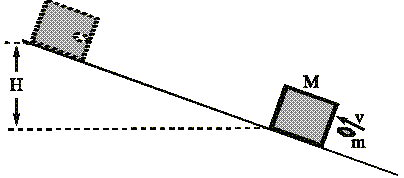
\includegraphics[scale=.6]{/Users/jgates/desktop/latex/pics/inclinebulletblock}
\end{floatingfigure}
 
{\bf \Large{\arabic{ProbNum}}} A bullet of mass $25~g$ is fired along an incline and imbeds itself quickly into a block of wood of mass $2.5~kg$. The block and bullet then slide up the frictionless $20^{\circ}$ incline, traveling a maximum distance of 3.5 meters up the incline. The block is kept from sliding down the incline initially by as small peg (not shown).

\bigskip
Determine the speed of the bullet just before it hits the wood.\paragraph{}
\noindent
\vfill

%\hfill 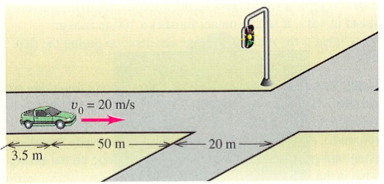
\includegraphics[scale=.85]{/Users/jgates/desktop/latex/pics/redlight.png}
\newpage